\chapter{Ancestry: how many histories, and what they hide}\label{ch:ancestry}

The first layer of generative information is the plainest: how many histories lead to an endpoint, and how the resulting uncertainty divides among the things one might want to know. This chapter proves that SELECT-II fibres are finite and nonempty, decomposes the ambiguity of an endpoint exactly into source, content, swap-class and within-class parts, works out the endpoint $72$ completely, and gives exact counts for the family $72^r$.

\section{Reverse edges and finite fibres}
For an integer $t\ge1$ write $s(t)=\prod_p p^{\lfloor v_p(t)/2\rfloor}$, where $v_p$ is the $p$-adic valuation, and $\tau(n)$ for the number of divisors of $n$.

\begin{proposition}[reverse edges and finiteness]\label[proposition]{prop:reverse-edge}\label[proposition]{prop:fibre-finite}
Let $t\ge2$.
\begin{enumerate}[label=(\alph*)]
\item There is an edge $m\xrightarrow{N}t$ iff $(N{+}1)^2\mid t$, and then $m=Nt/(N{+}1)^2$.
\item Every edge strictly increases the state: $t/m=N+2+1/N\ge4$, with equality iff $N=1$.
\item The number of reverse edges at $t$ is $\tau(s(t))-1$; the labels are $N=d-1$ for the divisors $d\ge2$ of $s(t)$.
\item A history from $m_0$ to $t$ has length at most $\lfloor\log_4(t/m_0)\rfloor$. In particular $F_t$ and $F_t(m_0)$ are finite.
\item An integer has a reverse edge iff it is not squarefree. Consequently every $t\ge1$ has at least one complete history, $|F_t|=1$ iff $A(t)=0$, and the counting recursion
\begin{equation}\label[proposition]{eq:recursion}
|F_t|=\begin{cases}1,& t\text{ squarefree},\\ \sum_{m\xrightarrow{N}t}|F_m|,& \text{otherwise}\end{cases}
\end{equation}
holds for complete-history fibres.
\end{enumerate}

\end{proposition}
\begin{proof}
(a) If $m\xrightarrow{N}t$ then $N\mid m$; write $m=kN$, so $t=kN(N{+}1)^2/N=k(N{+}1)^2$, which gives $(N{+}1)^2\mid t$ and $m=N\,t/(N{+}1)^2$. Conversely if $(N{+}1)^2\mid t$, put $k=t/(N{+}1)^2$ and $m=Nk$; then $N\mid m$ and $T_N(m)=k(N{+}1)^2=t$.

(b) $t/m=R(N)=N+2+1/N$ and $N+1/N\ge2$ with equality iff $N=1$ (AM--GM), so $R(N)\ge4$.

(c) By (a) the reverse edges correspond to integers $d=N{+}1\ge2$ with $d^2\mid t$. Writing $d=\prod p^{b_p}$, $d^2\mid t$ iff $2b_p\le v_p(t)$ for all $p$, iff $b_p\le\lfloor v_p(t)/2\rfloor$ for all $p$, iff $d\mid s(t)$. The divisors $d\ge2$ of $s(t)$ number $\tau(s(t))-1$.

(d) Each step multiplies the state by at least $4$ by (b), so a history of length $\ell$ ends at $t\ge4^\ell m_0$. For a fixed endpoint, backward steps from $t$ branch into finitely many predecessors by (c), each at least four times smaller, so the backward tree has depth $\le\log_4 t$ and is finite; histories ending at $t$ correspond to backward paths.

(e) By (c) $m$ has a reverse edge iff $s(m)>1$ iff some $d\ge2$ has $d^2\mid m$ iff $m$ is not squarefree. Existence of a complete history of $t$ follows by strong induction: if $t$ is squarefree, $(t;\,)$ is one; otherwise pick a reverse edge $m\xrightarrow{N}t$ ($m<t$ by (b)), take a complete history of $m$ and append $N$. A squarefree state has no reverse edge, so a complete history is a maximal backward path, and \eqref{eq:recursion} follows by splitting by the last label. Finally $|F_t|=1$ iff $\log_2|F_t|=0$.
\end{proof}

By part (e) every endpoint has at least one \emph{complete} history, i.e.\ one from a squarefree source, which is why $A(t)$ is defined for every $t\ge1$ (the \emph{complete-history convention}). For fixed-source fibres $F_t(m_0)$ may be empty, and $A(t\,|\,m_0)$ is then undefined; $\log_20$ is never written.

\section{Ambiguity and its exact decomposition}
The number $A(t)=\log_2|F_t|$ is the \emph{capacity} of ancestry: for any probability distribution on a fibre of size $N$ the entropy lies between $0$ and $\log_2N$, with the maximum attained exactly by the uniform distribution (Gibbs' inequality~\cite{CoverThomas}). A real process that weighs histories non-uniformly therefore has $\Ent(W|T=t)<A(t)$, and the gap is the information the weighting adds. Let $T$ be the endpoint, $M$ the source, $Q$ the content, $C$ the swap class and $W$ the history.

\begin{theorem}[hierarchy and decomposition]\label[theorem]{thm:hierarchy}
In a commutative realization with finite fibres and any ensemble,
\[
\Ent(W|T)=\Ent(M|T)+\Ent(Q|M,T)+\Ent(C|M,Q,T)+\Ent(W|C,T),
\]
and $\Ent(C|T)=\Ent(M,Q|T)+\Ent(C|M,Q,T)$. Under the uniform ensemble on a single fibre $F_t$, the left side is $A(t)$.

\end{theorem}
\begin{proof}
By \cref{lem:swap-invariants}, $T$ is a function of $(M,Q)$, $(M,Q)$ a function of $C$, and $C$ a function of $W$. If $X=f(Y)$, then $\Ent(Y|Z)=\Ent(X|Z)+\Ent(Y|X,Z)$ whenever $Z$ is determined by $X$ (chain rule). Apply this with $Z=T$ successively to $X=(M,Q)$, $X=C$ and $X=W$: $\Ent(W|T)=\Ent(M,Q|T)+\Ent(C|M,Q,T)+\Ent(W|C,M,Q,T)$. Since $C$ determines $(M,Q)$, $\Ent(W|C,M,Q,T)=\Ent(W|C,T)$. Finally $\Ent(M,Q|T)=\Ent(M|T)+\Ent(Q|M,T)$ by the chain rule once more. The second identity is the same chain-rule step applied to $C$. For the uniform ensemble on $F_t$, $\Ent(W|T=t)=\log_2|F_t|$.
\end{proof}
The four terms have clear meanings: $\Ent(M|T)$ is uncertainty about the seed, $\Ent(Q|M,T)$ about the multiset of operations given the seed, $\Ent(C|M,Q,T)$ about \emph{which reordering class} given seed and content, and $\Ent(W|C,T)$ is the residual order inside a class. The last is reordering ambiguity in the classical sense; the first three are structural.

\begin{proposition}[class entropy and component count]\label[proposition]{prop:class-entropy}
Under the uniform ensemble on a fibre with $N$ histories and recombination classes of sizes $n_1,\dots,n_k$ ($k=\beta_0(G_t)$),
\[
\Ent(C|T{=}t)=-\sum_i\tfrac{n_i}{N}\log_2\tfrac{n_i}{N}\le\log_2k,\qquad \Ent(W|C,T{=}t)=\sum_i\tfrac{n_i}{N}\log_2n_i\le\log_2n_{\max},
\]
with equality in the first iff all $n_i$ are equal, and $A(t)=\Ent(C|T{=}t)+\Ent(W|C,T{=}t)\le\log_2k+\log_2n_{\max}$.

\end{proposition}
\begin{proof}
The distribution of $C$ puts mass $n_i/N$ on class $i$, so its entropy is at most $\log_2k$ with equality iff uniform. Given $C=i$ the history is uniform on $n_i$ points, so $\Ent(W|C=i)=\log_2n_i$; average over $i$. The identity $A=\Ent(C)+\Ent(W|C)$ is the chain rule.
\end{proof}

\section{The endpoint 72}
\begin{example}[the endpoint 72]\label[example]{ex:72}
Since $72=2^3\cdot3^2$ we have $s(72)=2\cdot3=6$, so the reverse edges correspond to $d\in\{2,3,6\}$, i.e.\ to labels $N\in\{1,2,5\}$ with predecessors $18,\,16,\,10$ ($N=1$: $72/4$; $N=2$: $2\cdot72/9=16$; $N=5$: $5\cdot72/36=10$). Following predecessors:
\begin{itemize}
\item $10$ is squarefree: history $(10;5)$.
\item $18=2\cdot3^2$ has $s=3$, one reverse edge ($N=2$, predecessor $4$); $4$ has $s=2$, reverse edge $N=1$, predecessor $1$, squarefree: history $(1;1,2,1)$.
\item $16=2^4$ has $s=4$, reverse edges $N=1$ (predecessor $4$) and $N=3$ (predecessor $3$, squarefree). From $4$, as before, we reach $1$. Histories $(3;3,2)$ and $(1;1,1,2)$.
\end{itemize}
Hence $F_{72}=\{(1;1,1,2),\ (1;1,2,1),\ (3;3,2),\ (10;5)\}$ and $A(72)=2$ bits. The words $(1,1,2)$ and $(1,2,1)$ from source $1$ differ by a swap of adjacent distinct labels at the state $4$ and both are admissible (the states are $1,4,16,72$ and $1,4,18,72$): they form one class of size $2$; the histories of sources $3$ and $10$ have different sources and are isolated. The classes have sizes $2,1,1$. Under the uniform ensemble:
\begin{center}\small
\begin{tabular}{lcccccc}\toprule
$A(72)$ & $\Ent(M|T)$ & $\Ent(Q|M,T)$ & $\Ent(C|M,Q,T)$ & $\Ent(W|C,T)$ & $\Ent(C|T)$ & check\\\midrule
$2$ & $1.5$ & $0$ & $0$ & $0.5$ & $1.5$ & $2=1.5+0.5$\\\bottomrule
\end{tabular}
\end{center}
(sources $1,1,3,10$ with probabilities $\tfrac12,\tfrac14,\tfrac14$ give $\Ent(M|T)=1.5$; each source carries one content, so the two middle terms vanish). In the fixed-source fibres, $|F_{72}(1)|=2$ and $|F_{72}(3)|=|F_{72}(10)|=1$. A nonuniform ensemble such as $p=(\tfrac12,\tfrac14,\tfrac18,\tfrac18)$ gives $\Ent=1.75<2$.

\end{example}

\begin{figure}[ht]\centering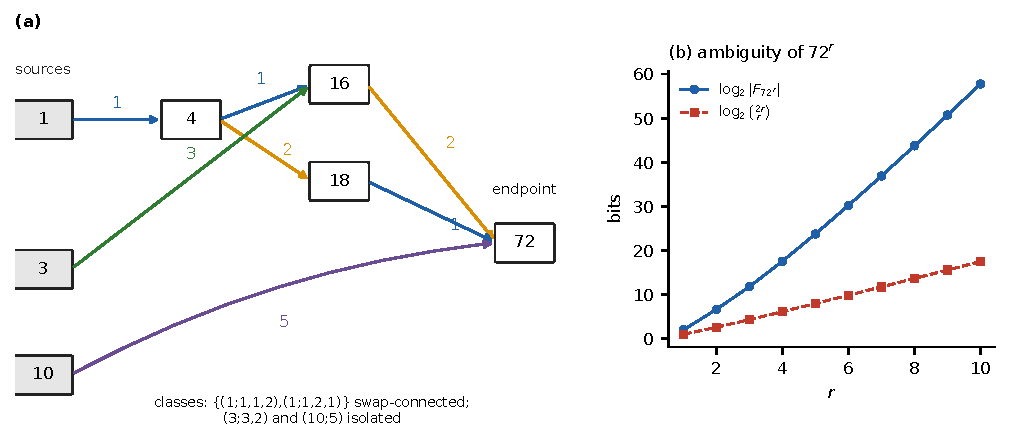
\includegraphics[width=\textwidth]{figures/fig_ancestry.pdf}
\caption{(a) The four histories of $72$ as paths of the arithmetic ancestry graph; edges carry their labels and shaded boxes are squarefree (complete) sources. The two histories from source $1$ differ by one legal swap, the labels $1,2$ at state $4$, and form a swap class; the histories from $3$ and $10$ are isolated classes. (b) Exact ambiguity $\log_2|F_{72^r}|$ against the proved lower bound $\log_2\binom{2r}{r}$ (\cref{prop:72r}).}\label{fig:ancestry}
\end{figure}

\section{Growth of ambiguity: the family \texorpdfstring{$72^r$}{72 to the r}}
How fast does ambiguity grow as the endpoint becomes richer? The simplest family is $t=72^r$, which contains a large block of independent-looking reorderings.

\begin{proposition}[growth of $72^r$]\label[proposition]{prop:72r}
(a) For every $r\ge1$, $|F_{72^r}|\ge\binom{2r}{r}$, hence $A(72^r)\ge\log_2\binom{2r}{r}$.
(b) The exact counts for $r=1,\dots,10$ are in \cref{tab:72r}.

\end{proposition}
\begin{proof}
(a) For $S\subseteq\{1,\dots,2r\}$ with $|S|=r$ let $w_S=1^r\,u$ where $u\in\{1,2\}^{2r}$ has $u_i=2$ iff $i\in S$. Start at the squarefree source $1$. Label $1$ is always admissible ($1$ divides every integer) and multiplies the state by $R(1)=4$, adding $2$ to the $2$-adic valuation $v_2$. Label $2$ multiplies by $R(2)=9/2$, subtracts $1$ from $v_2$, and is admissible iff the state is even. After the prefix $1^r$ the state is $4^r$, so $v_2=2r$; in the tail the $j$-th label $2$ ($j\le r$) is preceded by at most $j-1$ labels $2$, so $v_2\ge2r-(j-1)\ge r+1\ge1$. Every $w_S$ is therefore admissible. The label $1$ occurs $r+r=2r$ times and $2$ occurs $r$ times, so the endpoint is $R(1)^{2r}R(2)^r=4^{2r}(9/2)^r=72^r$. Source $1$ is squarefree, so each $(1;w_S)$ is a complete history of $72^r$, and different $S$ give different words.

(b) The counts are computed by the recursion \eqref{eq:recursion}, memoised on the exponent vector of the state.
\end{proof}
\begin{table}[ht]\centering\small
\begin{tabular}{rrrrr}\toprule
$r$ & $|F_{72^r}|$ & $A(72^r)$ (bits) & increment & $\log_2\binom{2r}{r}$\\\midrule
1 & 4 & 2.000 & --- & 1.000\\
2 & 100 & 6.644 & 4.644 & 2.585\\
3 & 3\,601 & 11.814 & 5.170 & 4.322\\
4 & 194\,864 & 17.572 & 5.758 & 6.129\\
5 & 14\,177\,856 & 23.757 & 6.185 & 7.977\\
6 & 1\,258\,011\,667 & 30.228 & 6.471 & 9.852\\
7 & 127\,958\,272\,791 & 36.897 & 6.668 & 11.745\\
8 & 14\,628\,387\,999\,697 & 43.734 & 6.837 & 13.652\\
9 & 1\,831\,257\,259\,071\,051 & 50.702 & 6.968 & 15.569\\
10 & 247\,547\,117\,576\,968\,617 & 57.780 & 7.079 & 17.495\\\bottomrule
\end{tabular}
\caption{Exact ambiguity of $72^r$ (complete-history fibres). Counts for $r\le7$ were recomputed exactly; the values for $r=8,9,10$ come from an earlier computation and were not repeated. The increments increase but with shrinking steps; no limit of $A(72^r)/r$ is claimed.}\label{tab:72r}
\end{table}
The bound is far from sharp: at $r=10$ it gives $17.5$ bits whereas the exact value is $57.8$, because the fibre contains, besides the reorderings of $1$'s and $2$'s from source $1$, many histories through other squarefree sources and other labels. Whether $A(72^r)/r$ converges is not known.

\section{Fixed-source and complete-history ambiguity}
The two fibre conventions differ: $A(t)$ counts all complete histories, whereas $A(t\,|\,m_0)=\log_2|F_t(m_0)|$ counts those from one seed. For $72$ the complete ambiguity is $2$ bits and the fixed-source ambiguities are $1,0,0$ bits for $m_0=1,3,10$; the missing information $\Ent(M|T)=1.5$ bits is the uncertainty about the seed. In general $A(t)\ge\max_{m_0}A(t|m_0)$ and $A(t)=\log_2\sum_{m_0}|F_t(m_0)|$.

\medskip
The decomposition of \cref{thm:hierarchy} organises everything that follows: the last two terms concern histories that differ only by legal swaps, which is the geometry of \cref{ch:swaps}; the first two concern which seeds and contents are admissible, which is the arithmetic of \cref{ch:arith}.
